\documentclass[12pt]{article}
\input{/home/dmitry/Work/Research/thesis/FINALE/settings.tex}
\graphicspath{{/home/dmitry/Work/Research/thesis/FINALE/INTRODUCTION/content/}}

%\documentclass[PhD_Thesis.tex]{subfiles}
\begin{document}

%\section*{Abstract}
%The surface and interior wave motions interact with the sea bottom irregularities altering gravity 
%wave energy propagation. Directional scattering and mode conversion will inevitably reshape a wave 
%field and will impel restructure of localized energy budgets. Here three geophysically important 
%cases are investigated: (1) a tsunami wave scattering from a prominent sea mount, (2) origination 
%of a semidiurnal internal tide and (3) reflection of the internal tide from a continental slope. 
%These problems are investigated by means of numerical experiments and theoretical analysis.\\
%A tsunami wave is scattered by Koko Guoyt such that amplified and delayed signals were observed 
%during recent tsunami events. The numerical simulations emphasize complicated response. The energy 
%focusing occurs in dependence to tsunami incidence angel and frequencies involved. Koko guoyt as 
%having asymmetrical shape selectively amplifies tsunami wave frequency. The provided theoretical 
%analysis further outlines regions and parameters which would lead to higher amplification.\\
%Internal tides originate from surface tide interaction with steep submarine ridges. This phenomena 
%undergoes temporal variation leading to nonstationarity in the far field. It is shown for Tasman 
%Sea that remote internal tide modulates magnitude of energy conversion. Further leading to spatial 
%variability many kilometers away.\\
%The Tasman Sea internal tides impinge on the continental slope partially reflecting. The 
%reflectance markedly depends on generation of along slope leaky mode. Under some conditions 
%coupling with the surface tide occurs leading to overall energy increase (additional source?) that 
%outgoing energy becomes larger than incident amount. This deviates from classical two dimensional 
%view on reflection/scattering process of the internal tides. The presented estimates of energy 
%transfers further emphasize large variability mainly coming from along slope topography 
%inhomogeneity.\\
%Results for the problems conspicuously show importance of three dimensional topographic structure 
%in order to describe wave energy propagation. This has strong effect on variability in the 
%resulting wave field and wave energy sinks.

\newpage
\section{Introduction}
Oceanic gravity waves fundamentally contribute to the redistribution of mechanical energy in the 
world ocean. Wave propagation can be altered as a result of interaction with large-scale 
sea bottom features such as submarine mountains, trenches and continental slopes. This 
modifies energy pathways by causing wave reflections or transformation of wave structure. In this 
work, by means of numerical simulations, these processes are examined for tsunamis and internal 
waves of tidal frequency (internal tides) for realistic cases of their interaction with ocean's 
bottom relief.\\
Tsunamis are transient waves that are impulsively forced by submarine earthquakes. The waves 
traverse vast expanses of the oceans and encounter numerous sea bottom features 
\citep{mofjeld2001tsunami}. In each instance, scattering redirects portion of incident energy. This 
process in case of the Hawaiian-Emperor seamount chain and Hess Rise leads to highly variable 
spatio-temporal tsunami impact on coastal regions \citep{kowalik2008kuril, tang2012direct}. First, 
this is characterized by wave trains arriving in an irregular sequence. The largest waves can 
unexpectedly appear with a several hour delay after an initial arrival 
\citep{koshimura2008effect}. At second, the overall wave intensity can markedly change along 
shorelines \citep{Borrero2013}. The problem of scattering by Koko Guyot, the largest submarine 
seamount in the Emperor chain (Figure 1), is investigated in the Chapter 1. The study intends to
quantify the interaction and the observed far-field signals in two recent tsunami events: the 2006 
Kuril and 2011 Tohoku-oki tsunamis.\\
The second problem considered in this dissertation explores internal waves that pervade the ocean's 
interior. Their existence depends upon water column stratification since these waves manifest as an 
oscillatory motion of isopycnal surfaces. The initial perturbation can be forced by different 
mechanisms: wind stress \citep{garrett2001near}, buoyancy flux \citep{garrett1979internal}, ice 
ridge keels \citep{morison1986internal} or even tsunami \citep{santek2007satellite}. Additionally, 
tidal currents at steep topography can excite internal waves. These are baroclinic waves 
that oscillate with tidal frequency and are called internal or baroclinic tides.\\
One reason to study baroclinic tides is their role in the dissipation of barotropic (surface) tidal 
energy \citep{munk1997once}. Current estimates suggest that 1/3 of total tidal energy is 
converted into internal motions in the deep ocean \citep{egbert2000significant}. From this roughly 
1/3 is directly lost to turbulent mixing right at generation sites \citep{st2002role} while the 
rest is emitted as freely propagating waves in form of tight beams \citep{simmons2004tidally}. 
These structures are observed to cross the ocean basins without much attenuation 
\citep{zhao2016global}. This finding fuels scientific research to understand where and how the 
baroclinic tidal energy is dissipated. Since the deposition sites primarily would occur deep below 
direct wind influence, the internal tides are thought to be a candidate for providing mechanical 
energy to close the upwelling branch of the Meridional overturning circulation 
\citep{munk1998abyssal}. Regardless of global importance, the baroclinic tides are relevant for 
local processes such as water mass transformation \citep{stigebrandt1989vertical}, vertical 
nutrient fluxes \citep{sharples2007spring}, sediment \citep{hotchkiss1982internal} and larvae 
transports \citep{pineda1999circulation}. All of the above is crucially dependent on an efficiency 
of energy removal in the process of internal-tide generation, propagation and scattering. 
At this point, respective parameterizations are in a premature state to have prognostic value.\\
In the setting of the Tasman Sea, an internal tidal beam originates at Macquarie Ridge and impinges 
on the continental slope of Tasmania (Figure 1). The Tidal Dissipation Experiment (TTIDE) had its 
goal to quantify the internal tide reflection and associated energy lost. This involves estimation 
of wave energy being reflected back into the open sea, converted into higher vertical modes and 
consequently, describe processes associated with sink of energy. These are the problems addressed 
in Chapters 2 and 3.\\
The two geophysical problems examined in the dissertation represent wave scattering by 
inhomogeneity in propagation media. Here, it takes form of a rapid bathymetric change
imposing constrains on fluid motions. Accompanying transformations are intrinsically linked to 
an energy flux approach. This is reviewed in \textbf{Section 2} of the Introduction by considering 
a normal mode dynamics, while \textbf{Section 3} describes energy characteristics associated with 
wave transformations caused by the interaction with bathymetry.\\

%physically based mixing parametrization

%Consequently, this provides insight for future parametrization 
%of internal tide reflection that would allow for energetically constrained internal wave 
%models (e.g. \citep{eden2014energy}.

%\textit{At such location the energy would drain into perturbations of isopycnals that further can travel hundreds of  leagues without any significant loss of energy. In the second part of my thesis origination, propagation and dissipation of the internal tidal beam is investigated on the example of Tasman Sea.\\
%A global internal tide model, satellite altimetry measurements and in situ observations indicate that a ridge south of New Zealand is a site for the generation of the strong tidal beam that is directed towards the Tasman Shelf break. The low mode internal wave beam undergoes scattering from topography, which transfers energy to shorter length scales. Thus, understanding of local energy processes will lead to a more detailed picture of tidal energy dissipation.\\
%\textbf{PLUGIN: 2 TW, 1 TW, Macquarie Ridge, internal tides produce transport of particulates: sediments and can cause strong currents in deep ocean. Role in tidal dissipation, Internal tides what became apparent recently are important energy transporters.}

\newpage

\section{Normal modes in a flat-bottom sea}
Tsunami and internal tides are long gravity waves. Their typical wavelengths are order of 
100 km being larger than the ocean's mean depth. Thus, the wave dynamics can be well described 
under the linear, hydrostatic framework. As a first step, wave propagation in a flat-bottom ocean 
is discussed. The equations of motion in stratified, Boussinesq ocean on an f-plane 
\citep{kundu2008fluid, cushman2011introduction} will take mathematical form of
\begin{subequations}
	\label{In:Beq}
	\begin{align}
	\pder[u]{t} - f v = -\frac{1}{\ib{\rho}_0}\pder[p]{x}\\
	\pder[v]{t} + f u = -\frac{1}{\ib{\rho}_0}\pder[p]{y}\\
	0 = -\pder[p]{z} - \rho g\\
	N^2 w = -\frac{1}{\ib{\rho}_0} \pderr[p]{z}{t}\\
	\pder[u]{x} + \pder[v]{y} + \pder[w]{z} = 0
	\end{align}
\end{subequations}
where $(u,~v,~w)$ are velocity along zonal, meridional and vertical axis, $f$ is the Coriolis 
parameter, $p$ is the perturbation pressure arising either from sea level oscillations or isopycnal 
displacements within stratified water column measured by Brunt-Vaisala frequency $N^2 = 
-\frac{g}{\ib{\rho}_0}\pder[\rho_0]{z}$. Additionally, boundary conditions are imposed on the 
surface and bottom as
\begin{align}
w|_{z = 0} = \pder[\zeta]{t},~p|_{z = 0} = \ib{\rho}_0 g \zeta\\
w|_{z = -H} = 0\label{In:bc.swe}
\end{align}
Both conditions are of linear form since the sea level motions are much smaller than the 
acceleration due to gravity, and the ocean depth is fixed. This formulation allows a solution via 
separation of vertical motions by employing following decomposition,
\begin{align}
(u, v, p)(x,y,z,t) = \sum_{n = 0} [u_n(x,y,t), v_n(x,y,t), p_n(x,y,t)]\psi_n(z)\\
w(x,y,z,t) = \sum_{n = 0} [w_n(x,y,t)] \int_{-H}^z \psi_n(z) dz\\
\rho(x,y,z,t) = \sum_{n = 0} [\rho_n(x,y,t)] \frac{d \psi_n(z)}{dz}
\end{align}
Upon substitution into \eqref{In:Beq} Sturm-Liouville problem is obtained for vertical structure 
(basis) functions $\psi_n(z)$\footnote{note this is for horizontal variables, usually it is written 
for vertical velocity since boundary conditions are expressed right away},
%\pder[\frac{1}{N^2 - \omega^2} \pder[\psi_n]{z}]{z} + \big(1 - \frac{f^2}{\omega^2} \big) \frac{\psi_n}{c^2_n} = 0
\begin{equation}
\frac{d}{dz}\big( \frac{1}{N^2} \frac{d \psi_n}{dz} \big) + \frac{1}{c^2_n}\psi_n = 0
\end{equation}
with an eigenvalue $c_n$ for a respective $n$-th vertical mode. $c_n$ is the wave phase speed in a 
non-rotating ocean with an equivalent depth, $D_n$ such that $\sqrt{g D_n} = c_n$. The 
decomposition separates vertical motions from horizontal dynamics reducing the initial set 
\eqref{In:Beq} to the Laplace tidal equations,
\begin{subequations}
\label{In:sweq}
\begin{align}
%\begin{split}
\pder[\vec{u}_n]{t} + f \vec{k} \times \vec{u}_n = -\frac{1}{\rho_0} \nabla p_n \label{In:swe.mom}\\
\frac{1}{\rho_0} \pder[p_n]{t} + g D_n \nabla  \cdot \vec{u}_n = 0 \label{In:swe.cont}
%\end{split}
\end{align}
\end{subequations}
This reveals the dynamical equivalence between barotropic, surface wave and baroclinic, internal 
waves if the ocean stratification were absent and the depth was $D_n$. In actuality, the $0$-th 
mode represents a barotropic solution with vertically uniform dynamics ($\psi_0 = const$) 
and the depth $D_0 \simeq H$ \citep{hendershott1981long}. The gravest mode represents pure surface 
wave propagation such as in the tsunami wave problem. The infinite sequence of higher vertical 
modes are internal modes that produce increasingly negligible sea level perturbations. This allows 
complete separation between barotropic and baroclinic motions which is similar to imposing rigid 
lid condition on internal modes \citep{kundu2008fluid}.\\
The main interest is in linear wave phenomena, so harmonic temporal behavior, $e^{i \omega t}$ 
will be imposed leading to the Helmholtz equation,
\begin{align}
\label{In:helmeq}
(\omega^2 - f^2) p_n + c_n^2 \Delta p_n = 0
\end{align}
Making a plane wave ansatz, $e^{-i\vec{k} \cdot \vec{x}}$, currents and pressure will be related as
\begin{align}
\begin{split}
p_n = p_{0n} e^{i (\omega t - \vec{k} \cdot \vec{x})}\\
u_n = \frac{1}{\ib{\rho}_0} \frac{\omega k_x + i f k_y}{\omega^2 - f^2} p_n\\
v_n = \frac{1}{\ib{\rho}_0} \frac{\omega k_y - i f k_x}{\omega^2 - f^2} p_n
\end{split}
\end{align}
Then from \eqref{In:swe.cont}, a dispersion relation for Sverdrup waves follows,
\begin{equation}
\omega^2 = f^2 + c^2_n |\vec{k}|^2
\end{equation}
The waves are dispersive as a result of Earth's rotation, with phase and group speeds are
\begin{align}
c_{p} = (1 - \frac{f^2}{\omega^2})^{-1/2} c_n,~c_g = (1 - \frac{f^2}{\omega^2})^{1/2} c_n,~c_p c_g 
= c_n^2
\end{align}
For temperate ocean stratification and deep ocean propagation, the most energetic mode-1 
semidiurnal internal tide phase travels with speed of $4~m/s$, but group speed is only $2~m/s$. So 
slow traveling wave is potentially affected by background oceanic circulation. On contrary, tsunami 
waves exhibit shallow-water, nondispersive behavior with phase and group speeds of $\sim 
O(100~m/s)$ owing to small periods in comparison to the Earth's rotation period. Tsunami waves 
cross ocean basins in a matter of hours without any appreciable interaction with ocean's dynamical 
state.\\
In the deep ocean, where the bottom topography does not demonstrate large spatial gradients, normal 
modes are useful to describe wave dynamics. An energy equation can be developed from 
\eqref{In:sweq}. Multiplying the momentum equations by $\vec{u}_n$ and the continuity equation by 
$p_n$, after adding both expressions and depth averaging one obtains the energy conservation law 
per each mode $n$,
\begin{equation}
(E_k + E_p)_t + \nabla \cdot \vec{F} = 0 \label{In:eneq}
\end{equation}
The horizontal energy flux is defined by
\begin{equation}
\vec{F}_n = \frac{1}{H} \vec{u}_n(t) p_n(t) \int_{-H}^0 \psi^2(z) dz \label{In:fldef}
\end{equation}
For tsunami wave propagation due to barotropic nature $\psi(z) = const$ and $p_n = \rho_0 g 
\eta$, the expression takes its classical form for surface wave propagation 
\citep{henry2001representation}, $\vec{F} = \rho_0 g \vec{u} \zeta$.\\
In internal tide studies period averaging further simplifies calculations,
\begin{align}
\vec{F}_n = \frac{1}{2H} \cj{\vec{u}}_n p_n \int_{-H}^0 \psi^2(z) dz
\end{align}
where velocity and baroclinic pressure are now complex amplitudes of a harmonic fit and $\cj{}$ is 
a complex conjugate.\\
The obtained expressions for the energy flux comprises only the pressure-work term, i.e. transport 
of energy is dictated by pressure forces. In the full formulation this is augmented with nonlinear 
contributions made by advection and dissipative forces \citep{gill2016atmosphere}. These terms 
are negligible presuming deep ocean propagation where wave's spatial dimensions are large and 
magnitude of dynamical variables is small.\\
%\citep{kang2012energetics}, \citep{nash2012unpredictable}
Away from scattering regions, an energy budget can be constructed following the linearized normal 
mode dynamics. Any loss in intensity of primary wave has to be balanced by energy scattered into 
other form of motion such as vertical modes or trapped waves and by dissipative losses. The latter 
is not discussed here and thought to constitute a residue term. The scattered wave field, 
reflected components and intermodal conversion are the main topic of investigation. The 
quantitative aspects are discussed in \textbf{Section 3}.\\

\section{Oceanic wave scattering}
Wave scattering in the ocean can be defined the same as for sound waves \citep{Lighthill2001}. The 
scattered component is said to be the difference between two wave fields:
\begin{itemize}
	\item the disturbed field when an inhomogeneity such as a change of underlying topography is 
	present and affects an incident wave;
	\item the field when the inhomogeneity is absent, so that it is given by the incident wave 
	only.
\end{itemize}
The difference arises solely because of the full bottom boundary condition,
\begin{equation}
( \vec{u} \cdot \nabla h )|_{z = -h(x, y)} = 0~\text{or}~w = - \vec{u}_h \cdot \nabla h 
\label{In:bcnon} 
\end{equation}
The condition states that there is no mass transport across an impermeable bottom. Incident wave 
motions cannot alone satisfy (\ref{In:bcnon}), and a compensating flow has to develop to preserve 
mass. For instance, when a wave train encounters a vertical wall in a nonrotating ocean, 
a specular reflection occurs in order to fulfill the no-flow condition.\\
An additional condition is imposed on scattered waves such that their energy vanishes with distance 
\citep{mei1989theory, morse1946methods, olbers1981formal}. The Sommerfeld radiation condition leads 
to a far-field asymptotic on a horizontal plane:
\begin{equation}
\label{In:def.scamp}
p_{scat} \sim \frac{e^{i \vec{k} \cdot \vec{x}}}{|\vec{x}|} \Phi_s (\theta)
\end{equation}
This is an assertion for circularly spreading waves having some angular distribution $\Phi_s$, 
called a scattering amplitude.\\
In the near-field, a scattered wave field can be decomposed by Fourier transform whereby each 
wavenumber can be regarded as a separate component. As it propagates away, it will begin to 
separate from others. Magnitude modulations due to interference \footnote{more appropriate to say 
diffraction} will subdue. And at large distances, respective Fourier coefficient will represent a 
scattering amplitude in direction corresponding to the wave vector. As a result, Fourier transform 
depicts the far-field's distribution of energy.\\
These are the general concepts of scattering phenomena. Since in this work two types of 
wave oscillations are dealt with, additional, specific comments follow.

\subsection{Tsunami wave scattering}
Since tsunamis are typical long, barotropic waves, the full nonlinear boundary condition can be 
incorporated into \eqref{In:swe.cont} to produce
\begin{equation}
\pder[\eta]{t} + \nabla  \cdot (H \vec{u}) = 0 
\end{equation}
When a tsunami encounters a topographic feature, a flow convergence due to the sloping bottom will 
cause localized reflection and reorientation of the motion. As a result, the topography will emit 
radially spreading waves. And the disturbed field will have an angular distribution distinct from 
the initial wave. Then the scattering amplitude will be a primary characteristic in the 
tsunami-topography interaction \footnote{\citep{vastano1973transient, saito2009scattering}}.\\
Because of tsunami's transient nature, the interaction will also transfer energy into trapped 
motions \citep{longuet1967trapping, tinti1995tsunami}. They usually thought as standing 
waves\footnote{ or ``sloshing modes"} associated with the topography's shape or as edge waves 
confined to the slope. Such transient trapped waves do significantly contribute to local 
oscillations as slowly re-emitted energy leaks into the open ocean, but in the far-field this will 
not have appreciable effect.\\
For long wave scattering it is usually possible to simplify discussion by omitting some topographic 
variations such as an exact slope profile. It is then considered to be a depth discontinuity. So 
that, a seamount, such as Koko Guyot, will be analogous to a cylinder. An error in wave dynamics of 
such representation decreases as $O(k^2 H^2)$ \citep{mei1989theory}, for the typical mean ocean 
depth's of 4000 m and wave periods longer than 10 minutes, the above simplification is valid. In 
this case, the nonlinear problem of \eqref{In:bcnon} is similar to fulfilling so-called matching 
conditions. These are mass conservation and continuity of sea level
\begin{align}
\vec{u}_1 h_1 = \vec{u}_2 h_2,~\zeta_1 = \zeta_2
\end{align}

\subsection{Internal tide scattering}
In the internal tide problem, in addition to the spatial energy redistribution, there could occur a 
transfer of energy into different vertical modes. This process is usually referred to as scattering 
in internal tide studies \citep[e.g.][]{muller1992scattering}. Let us consider a long wave that 
obeys Laplace tidal equations entering a region where bottom slope is inclined and the full 
boundary condition \eqref{In:bcnon} has to be satisfied. It only can be fulfilled if there is a 
vertical velocity. A normal mode by itself is not able to represent the dynamics since the vertical 
derivative, by definition, is zero on the boundary. However, a superposition of modes can force 
horizontal convergence to cancel out the vertical velocity. Physically, pressure gradients should 
develop by displacing isopycnal surfaces which further radiate energy away in the form of 
baroclinic modes. In general, this describes a coupled-mode approach \citep{griffiths2007internal}. 
Locally-flat normal modes counteract one another through the boundary condition. The spatial 
gradients will dictate mode's magnitude to ensure a balance. Dynamically, the Laplace tidal 
equations for each separate mode will embrace an additional force represented as an 
intermodal-coupling term \citep{griffiths2007internal, kelly2016coupled}.\\
Intermodal conversion and energy flux carried by modes can be estimated as work done by 
vertical velocity against modal pressure, $W_{m \to n} \sim (w_{m,~scat}~p_n)|_{z = 
-h} = -((\vec{u}_m \cdot \nabla h) p_n)|_{z = -h}$. But total conversion must as well account for 
the opposite energy transfer, from $n$ to $m$, hence,
\begin{align}
\label{In:en.trans}
C_{m \to n} = -((\vec{u}_m \cdot \nabla h)~p_n)|_{z = -h} + ((\vec{u}_n \cdot \nabla h)~p_m)|_{z = 
-h}
\end{align}
Internal tide excitation can be viewed as scattering of barotropic tide by a steep relief into 
higher (baroclinic) modes \citep{hendershott1981long}. If the surface tide is the $0^{th}$ mode, 
then energy lost can be diagnosed as
\begin{align}
\label{In:bt_bc}
C_{bt \to bc} = -(\vec{u}_{bt} \cdot \nabla h)~\sum_{n = 1} p_n|_{z = -h}
\end{align}
assuming that the baroclinic wave field effect on surface tide is negligible 
\citep{kelly2012cascade}. The above expression is well established in internal tide studies 
\citep{kurapov2003m, llewellyn2002conversion, pickering2015structure}.\\
For consideration of mode-1 scattering it is useful to reformulate \eqref{In:en.trans} by employing 
Leibniz's rule, the continuity equation per each normal mode, and mode's orthogonality,
\begin{align}
\label{In:bc_bc}
C_{m \to n} = \int_{-h}^{0} (u_m \nabla p_n - u_n \nabla p_m) dz
\end{align}
In the problem of internal wave propagation over uniform and gently inclined bottom 
\citep{wunsch1968propagation}, there is no intermodal conversion, $C_{m \to n} = 0$, and each 
mode's dynamics is perfectly matched by presence of others. Strictly speaking, in this case the 
wave equation is hyperbolic \footnote{(in contrary to elliptical Helmholtz equation, 
\eqref{In:helmeq})} and propagation occurs along characteristics \citep{sandstrom1969effect} or 
internal wave rays described by
\begin{equation}
\label{In:ch.angle}
\gamma = \frac{dz}{dx} = \pm \frac{\omega^2 - f^2}{N^2 - \omega^2}
\end{equation}
Slope criticality can be defined as the ratio of bottom gradient to rays angle, $\gamma$. In the 
subcritical regime of forward propagation, the ratio is less than unity. In this regime a more 
inclined bottom requires a greater number of modes to describe internal tide dynamics (Figure 
2). Now it is apparent that mode conversion will not happen, unless there is a change in the 
inclination to drive adjustment of mode amplitudes. In contrast, in the supercritical regime, when 
$\nabla h > \gamma$, internal waves are always reflected with increase of higher mode contribution. 
Usually, they will be phase-locked into vertically propagating rays \citep{garrett2007internal, 
lamb2014internal} subject to breaking and dissipation \citep{lien2001observations, 
nash2004internal, klymak2011breaking}. In case of a continental slope this causes internal tide 
mode-1 reflection to decrease relative to the equivalent case of surface wave reflection.\\
A similar to the tsunami problem simplification can be made by representing a topographic variation 
as a depth jump \citep{st2002role, larsen1969internal, chapman1981scattering}. \footnote{Should I 
mention no justification?} Now the matching conditions will require continuity of pressure across 
the jump and no momentum transport through vertical walls:
\begin{align}
p_1 = p_2, -h_2 \leq z \leq 0 \\
\vec{u}_1 = 0, -h_1 \leq z \leq -h_2\\
\vec{u}_1 = \vec{u}_2, -h_2 \leq z \leq 0
\end{align}

\section{Organization of dissertation and Novelty of investigation}
The thesis consists of three chapters. In each part wave-topography interaction is addressed for  
distinct geophysical settings. To summarize the topics and clarify terminology following table is 
given, as well necessary points are made in words.

\begin{table}
	\centering
	\begin{tabular}{ |M{3.5cm}|M{4.5cm}|M{4.5cm}|M{4.5cm}|  }
	\hline
	~ & Chapter 1 & Chapter 2 & Chapter 3\\
	\hline
	Topic & Tsunami propagation & Generation of an internal tidal wave & Reflection of a mode-1 
	internal tide\\
	\hline
	Scattering phenomena & Angular redistribution of wave energy & Conversion of barotropic tide 
	into baroclinic tide & Conversion of the gravest baroclinic mode into higher modes\\ 
	\hline
	Scattering diagnostic & \eqref{In:def.scamp} & \eqref{In:bt_bc} & \eqref{In:def.scamp} \& 
	\eqref{In:bc_bc}\\
	\hline
	Area & Koko Guoyt, Emperor Seamount Chain & Macquarie Ridge, New Zealand & Tasmania Continental 
	Slope\\
	\hline
	\end{tabular}\\
\caption{Overview of the dissertation}
\end{table}
	
\begin{enumerate}
	\item[Chapter 1] makes its goal analysis of scattering of tsunami waves by Koko Guyot. The 
	approach is based on obtaining scattering amplitude \eqref{In:def.scamp}, evaluation of its 
	frequency and spatial characteristics in order to describe far-field signals. The discussion 
	and conclusions are supported with analytical calculations based on matching conditions 
	approach.
	\item[Chapter 2] deals with generation of semidiurnal internal tide at Macquarie Ridge,  
	Tasman Sea. This is studied in a detail by analysis of three dimensional structure of 
	internal wave field. The proposed mechanism explains peculiarities of conversion rates 
	\eqref{In:bt_bc}. The emitted internal tidal beam than described in the far-field with emphasis 
	on its kinematic properties.
\textbf{Simple statement: generation of internal tides is affected by the remote signal -> 
this progresses into far-field.}
	\item[Chapter 3] concerns the tidal beam reflection from Tasman Continental Slope. The 
	obtained energy levels show variability that is due to number of factors. Possibility of each 
	is discussed and respective estimates are made in order to propose physically reasonable 
	mechanism of internal tide dynamics in three dimensionally complex region.

\end{enumerate}
Throughout the thesis a method based on inverse modeling was used. Its mathematical rudiments are 
given in Appendix A.

\section*{Figures}
\begin{figure}
	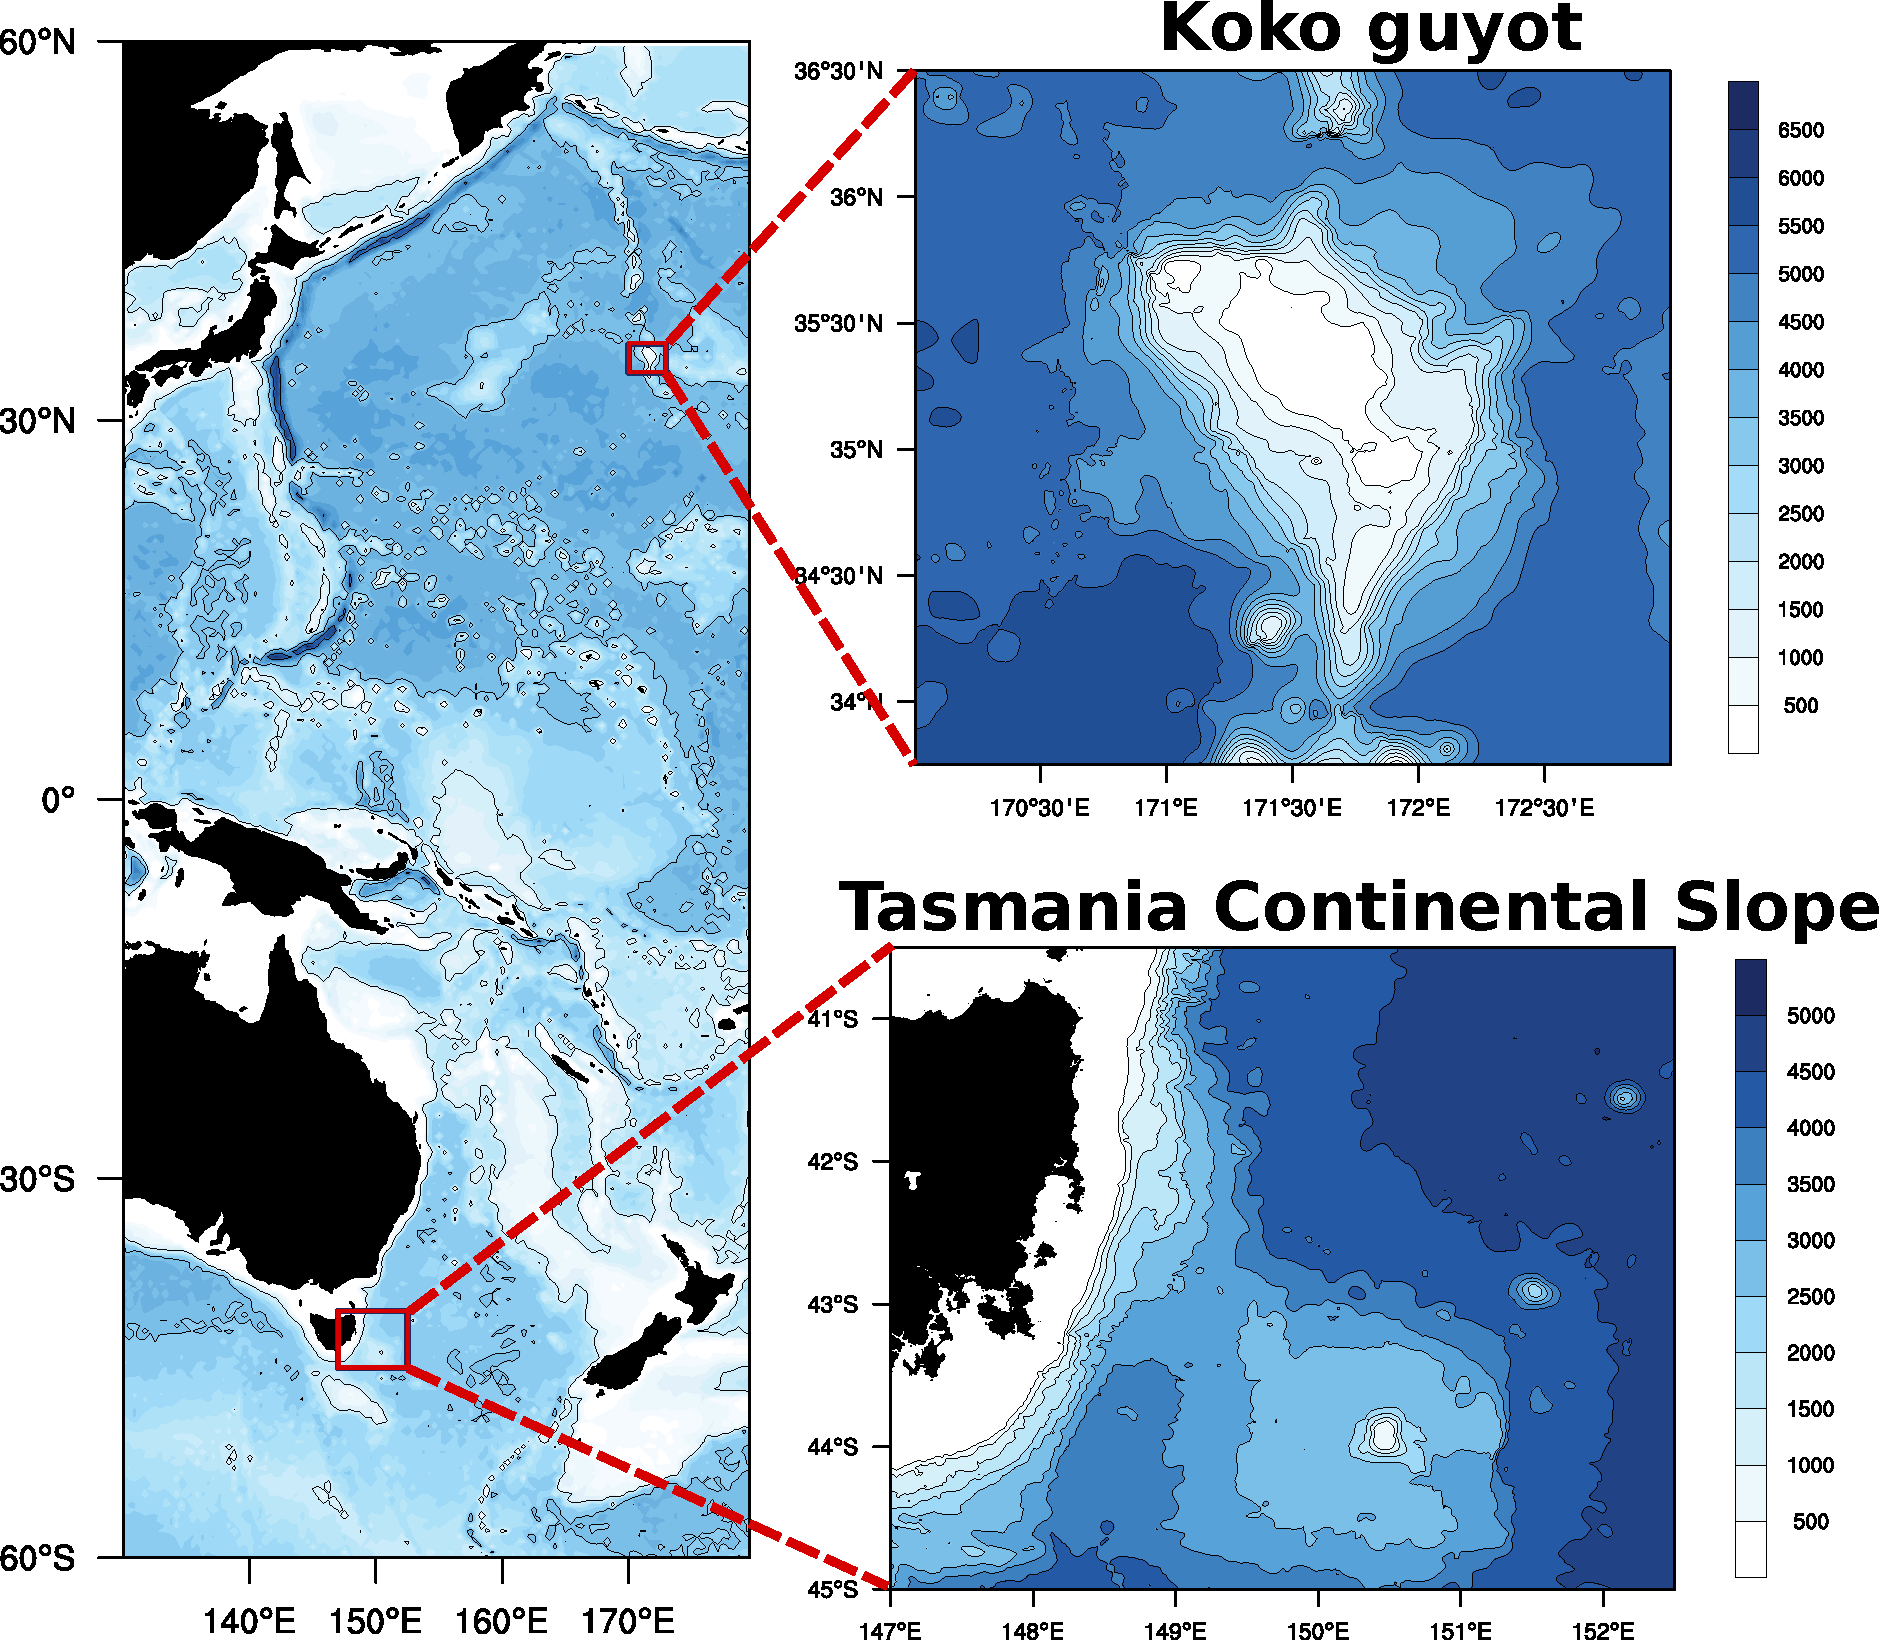
\includegraphics[scale=0.5]{/home/dmitry/Work/Research/thesis/FINALE/INTRODUCTION/figures/map_w_places.pdf}
	\caption{Bathymetric map of the Pacific Ocean with outlined regions showing geographic 
	locations of considered wave scattering problems.}
\end{figure}
	
\begin{figure}
	\includegraphics[scale=0.8]{/home/dmitry/Work/Research/thesis/FINALE/INTRODUCTION/figures/errors2.pdf}
	\caption{Error in description of internal wave structure by flat-bottom vertical modes as 
	bottom gets steeper \citep{wunsch1968propagation}.}
	%\includegraphics[scale=0.5]{../}
\end{figure}
%In overall, this thesis intends to investigate scattering process in three geophysical cases. In order to study this phenomena one will inevitably encounter interference which can lead to impossibility of direct energy budget estimates. Here I concerned with obtaining characteristics of how much energy was lost and how that energy was distributed in space. So decomposition of interference into elemental waves should be considered.\\
%I address this question by studying results of numerous numerical experiments with varying conditions. Hence, inconstancy of the tidal beam characteristics and its intertwine with topography and background conditions could be quantitatively described in order for better explanation of TTIDE field measurements.
% 
%\begin{enumerate}
%\item Chapter 1. Method for interference decomposition in numerical experiments on wave scattering.
%In order to quantify things such as directional distribution and reflection coefficient the field should be decomposed in order to obtain energy characteristics.
%
%\item Chapter 2. Scattering of tsunami waves by Koko Guyot.
%\item Chapter 3. Generation, structure and variability of Tasman internal tidal beam.
%\item Chapter 4. Reflection and scattering of the internal tidal beam by Tasman continental slope.
%%\item Chapter 5. Formal solution of scattering problem in framework of coupled Laplace tidal equations.
%\item Discussion, Conclusions, Future Work.
%\end{enumerate}


%occurring 
%Energy conservation, \eqref{In:eneq} sets an useful framework for analysis of the wave interaction 
%with topography. As bottom slope starts rapidly change, wave propagation undergoes variation 
%resulting in reorientation of currents, divergence in water column. But because of energy 
%conservation, amount of total energy should be preserved. Hence, energy transports of energy 
%through control volumes can present a valuable tool for description of wave interaction with 
%bottom 
%relief. The approach 
%
%I deliberately abandon nonlinear terms . Koko Guoyt depth on 
%average is around 500 m, barotropic velocity is of order $0.1~m/s$, nonlinear terms scale as $\sim 
%u^3$, while linear energy flux as $\sim g u \zeta$. It suggests that only in shallow water where 
%horizontal acceleration is of order of gravity acceleration, nonlinear terms will be a significant 
%addition to total energy transports. The same discussion on nonlinear additions stays true for 
%internal tide scattering from the Tasman continental slope which depth does not exceed $100~m$. 
%Only on shallow shelfs advection of kinetic energy becomes non-negligible 
%.\\

\newpage

\bibliographystyle{apacite}
\bibliography{/home/dmitry/Bibtex_lib/my_first_lib}

\end{document}